\documentclass{article}
\usepackage{graphicx}
\graphicspath{ {./Images/} }

\title{Crane Robot}
\author{Bogdan Stefan, Fleser Mihai, Presecan Alexandru}

\begin{document}
	\maketitle
	\vspace*{\fill}
	Group: 30434 \par
	Professor: Fuzes Attila
	\newpage
	
	\tableofcontents
	\newpage
	
	\section{Abstract}
	
	My colleagues and I decided to build a robot that had a robotic arm in order to challenge both our hardware and software skills. We had most of the parts on hand from previous projects. We learned a lot from building this robot, broadening both our electronics and software developing skills in the process. \\
	
	The robot is controlled by phone, and uses 4 DC motors, connected to Omni-Wheels for propulsion. The "brain" of the robot is an Arduino Uno, equipped with a shield used to control the robotic arm, attached to the upper part of the chassis. For power, we used 3 rechargeable lithium-ion batteries, as well as 2 voltage dividers, in order not to overload the Arduino. \\
	
	The chassis is made out of aluminium, which was cut and painted by us.
	
	\section{Components}
	
	\begin{itemize}
		\item 1 Arduino Uno development board, equipped with a shield
		\item 1 Arduino Bracio robot arm
		\item 4 DC motors
		\item 2 H-bridges
		\item 4 Omni-wheels
		\item 2 Voltage dividers
		\item 1 Voltage raiser
		\item 3 Li-ion batteries
		\item 1 Bluetooth receiver
		\item 1 Switch
		
	\end{itemize}
	
	\section{Schemas}
		
		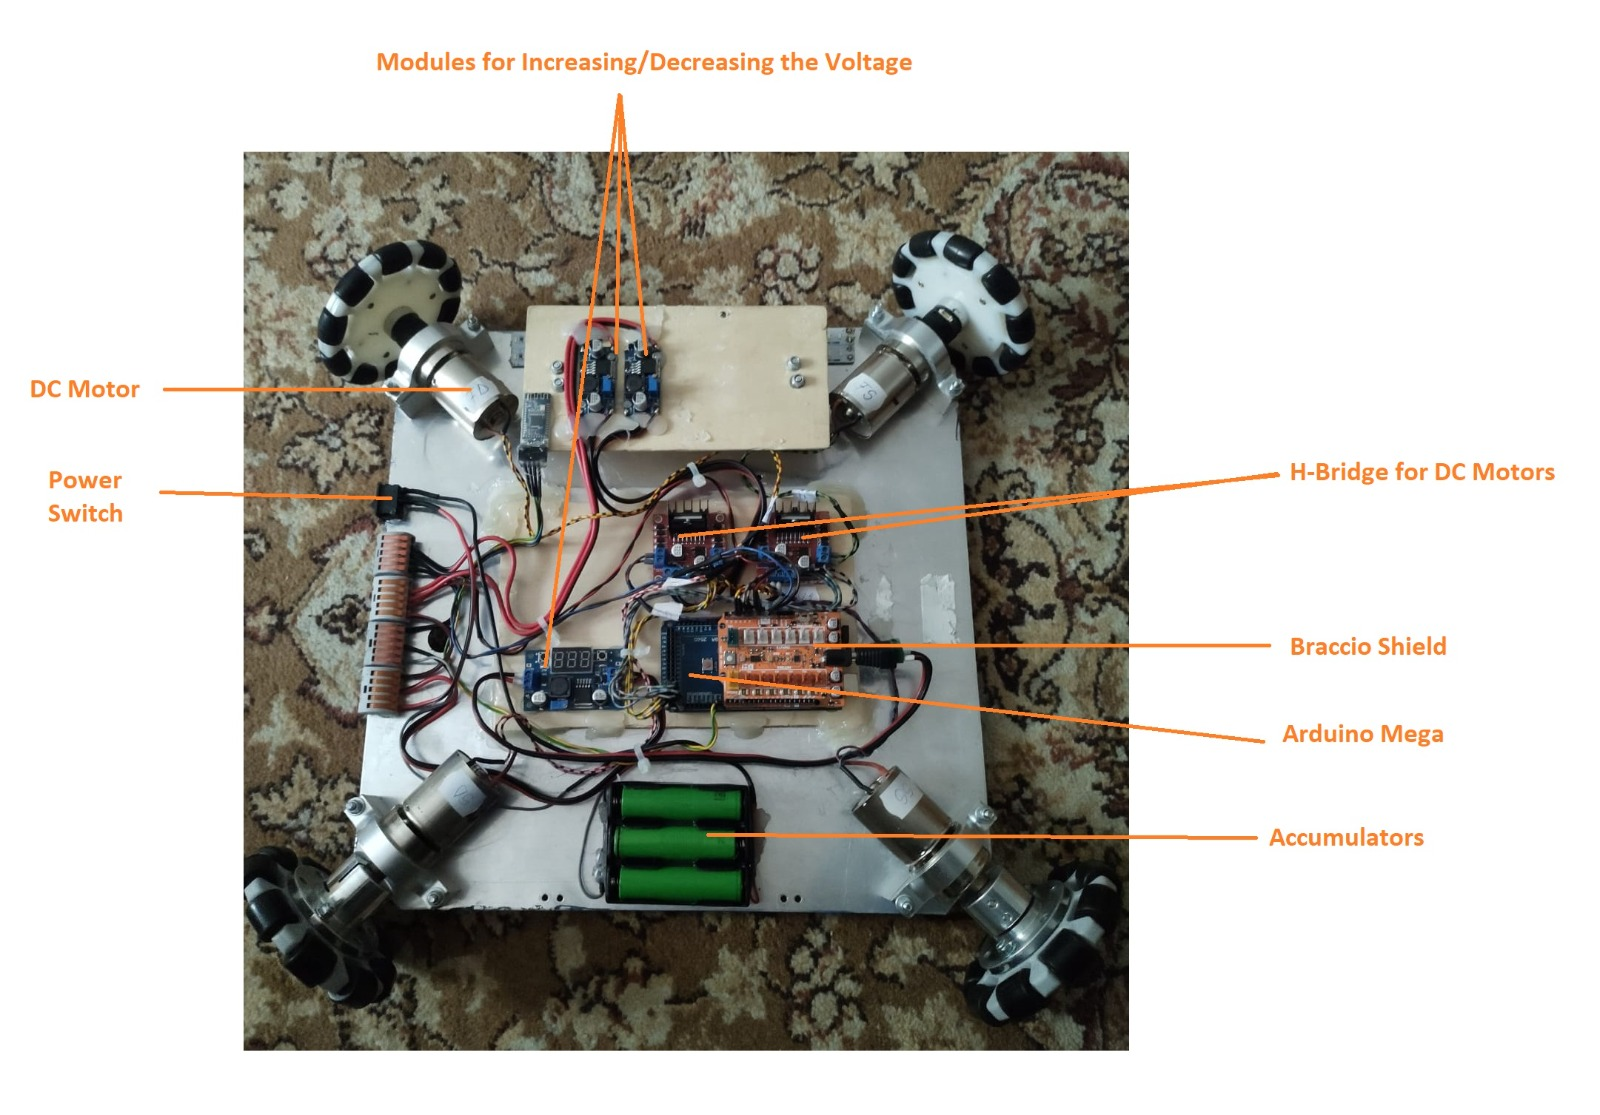
\includegraphics[scale = 0.25s]{mountingScheme.jpeg}
	
	\section{Program Flow}
	The code mostly consists of functions used to define both arm and wheel movement.\\
	
	The setup function is used to define the motors from the above-defined classes, as well as to initialise the serial monitor, the robot arm, and Dabble.
	
	The loop function handles phone inputs, and calls appropriate functions, depending on the user input, as well as the controller mode (arm or wheel).
	
	
	\section{Code}
	The code is too long to be included here, so we will include it in an archive.
	
\end{document}